\documentclass[12pt]{article} % For LaTeX2e
\usepackage{nips15submit_e}
\usepackage{times}
%\setmainfont{Times New Roman}
\usepackage{hyperref}
\usepackage{url}
\usepackage{graphicx}
\usepackage{dirtytalk}
\usepackage{float}
\usepackage{color}
\usepackage{amsmath}
\usepackage{caption}
\usepackage{multirow}
%\documentstyle[nips14submit_09,times,art10]{article} % For LaTeX 2.09


\title{Movie Classification Project - Final Report}

\author{
Jiejun Lu, Hongxiang Qiu, Weidong Xu, Zeyu Zhao\\
AC209B Group \#18\\
Harvard University\\
}

\newcommand{\plh}{\textbf{\color{red} PLACEHOLDER }}
\nipsfinalcopy % Uncomment for camera-ready version

\begin{document}

\maketitle

\section{Problem Statement and Motivation}

In this project, we implemented several machine learning models to predict the genres of movies using their {\bf overview descriptions and posters} (since we want to predict genres for new movies, we didn't use features like {\it ratings}, which are not available for new movies). We further compared those models and made a machine learning pipeline for the best model. {\bf The best model is a concatenated model composed of an encoder for posters and an encoder for overview texts}.

Our pipeline can be used to automatically tag the genres of movies on movie-hosting websites like Netflix and movie-database websites like TMDB.

{\bf All code for scraping data and building the models are submitted with this report.}

\section{Introduction and Description of Data}

In 2016, 736 new movies were released in US cinemas \cite{web_movie_num}, with more on websites like Netflix and YouTube. And the number of new movies released each year is still growing. Therefore, movie genre classification, which helps people quickly find the movies they want to watch, becomes more and more important.

In our project, we built machine learning models to automate the movie genre classification task. The input features for our models are the overview description texts and poster images of movies and the outputs are the predicted genres of the given movies.

The first step of building any machine learning model is obtaining the training and test datasets. For this project, we scraped all 361,622 movies from TMDB using the python library {\it tmdbsimple}. As for data cleaning, we removed movies with short overview length (less than 10 words) since the majority of them are empty/'No Overview'/'Not found'/ etc., or not enough to describe the movie. We also removed movies without available posters as we would like to integrate poster information to our final model. We are interested in recent movies, so after data cleaning, we only kept the latest 30,000 movies, including their overview descriptions, poster images and ground truth genres. For TMDB dataset, there are $19$ possible genres in total.

Before building our models, we performed the exploratory data analysis (EDA) and got some noteworthy findings on our data. Fig.~\ref{fig:hist} shows the histogram of the count of movies in corresponding genres. We can see the dataset is unbalanced. And intuitively, a movie can have multiple genres. For example, the well-known {\it Titanic} movie has genres {\it drama, romance and thriller}. Fig.~\ref{fig:co-occurrence} shows how genres appear together. It makes intuitive sense to see certain "exciting" categories group together, including crimes, horror, mystery, thriller, and "uplifting" categories group together, including animation, fantasy, family and adventure.

We also examined whether the overview descriptions and posters can be used to predict genres. Fig.~\ref{fig:poster-dif} below shows posters for a documentary movie (left) and an animation movie (right). We can see their styles are pretty different. Fig.~\ref{fig:word-cloud} shows the word cloud we generated for crime movies (top) and romance movies (bottom). We can see their key words are different ("Crime" v.s. "Love"). Therefore, we believe both the posters and overview descriptions can be useful to predict genres of movies.

\begin{figure}[H]
\centering
\begin{minipage}{0.5\textwidth}
  \centering
  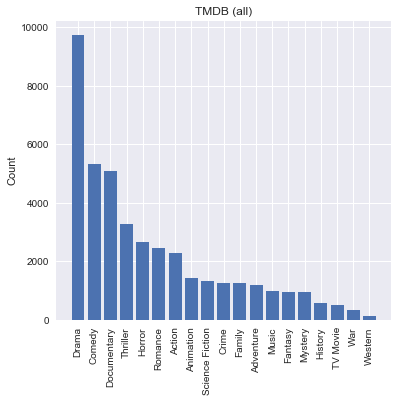
\includegraphics[width=\linewidth]{count.png}
  \caption{Histogram of Movie Genres}
  \label{fig:hist}
\end{minipage}%
\begin{minipage}{0.5\textwidth}
  \centering
  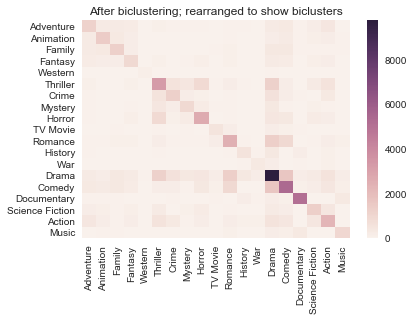
\includegraphics[width=\linewidth,height=7cm]{coappear.png}
  \caption{Co-occurrence of genres}
  \label{fig:co-occurrence}
\end{minipage}%
\end{figure}

\begin{figure}[H]
\centering
\begin{minipage}{0.5\textwidth}
  \centering
  \begin{minipage}{0.5\textwidth}
    \centering
    
\includegraphics[width=0.98\linewidth,height=7cm]{poster.png}
  \end{minipage}%
  \begin{minipage}{0.5\textwidth}
    \centering
    
\includegraphics[width=0.98\linewidth,height=7cm]{poster1.png}
  \end{minipage}%
  \caption{Posters for Different Genres}
  \label{fig:poster-dif}
\end{minipage}%
\begin{minipage}{0.5\textwidth}
  \centering
  \begin{minipage}{\textwidth}
    \centering
    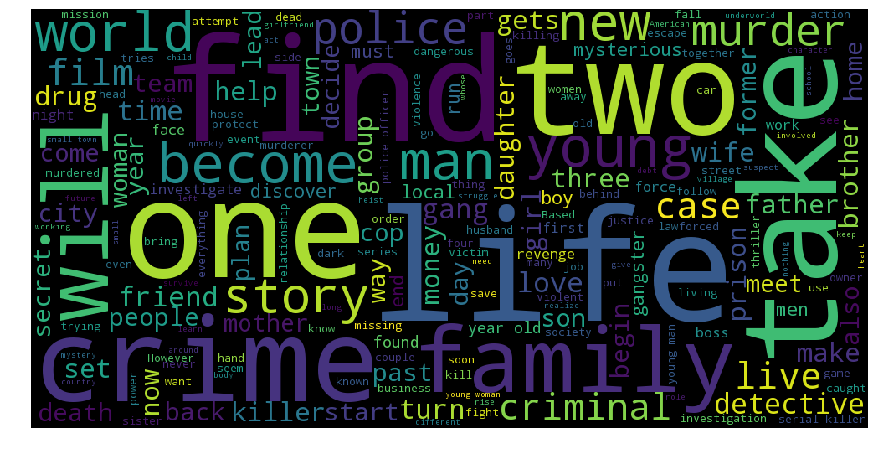
\includegraphics[width=\linewidth]{wordcloud.png}
  \end{minipage}
  \begin{minipage}{\textwidth}
    \centering
    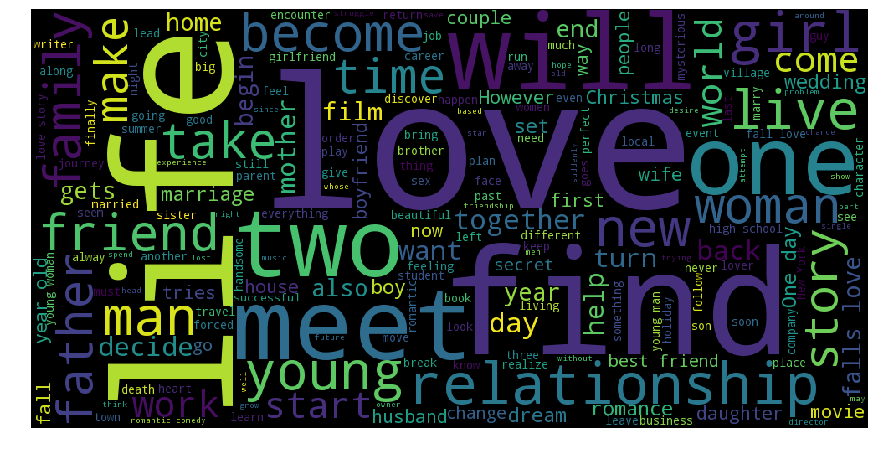
\includegraphics[width=\linewidth]{wordcloud1.png}
  \end{minipage}
  \caption{Word Cloud of Different Genres}
   \label{fig:word-cloud}
\end{minipage}%
\end{figure}

As aforementioned, movie genre classification is a multi-label classification problem. For models solving such problems, evaluation metrics for binary problems can not be easily applied (for example, if using AUC, we will now have $19$ values for all categories instead of $1$, and thus we can't rank our models easily). Previous work \cite{multilabel,multilabel1,multilabel2} used $F_1$-score (also called $F$-score or $F$-measure) as the evaluation metric. In our project, we choose {\bf micro averaged $F_1$-score} \cite{multilabel} as the metric. The equations for calculating the micro averaged statistics are:

\begin{equation} \label{eq:micro}
\begin{cases}
\text{Precision: }P_{micro}=\frac{\sum_{j=1}^k\sum_{i=1}^nY_i^jZ_i^j}{\sum_{j=1}^k\sum_{i=1}^nZ_i^j}\\
\text{Recall: }R_{micro}=\frac{\sum_{j=1}^k\sum_{i=1}^nY_i^jZ_i^j}{\sum_{j=1}^k\sum_{i=1}^nY_i^j}\\
F_{1-micro} = \frac{2\sum_{j=1}^k\sum_{i=1}^nY_i^jZ_i^j}{\sum_{j=1}^k\sum_{i=1}^nZ_i^j+\sum_{j=1}^k\sum_{i=1}^nY_i^j}
\end{cases}
\end{equation}

$Y_i^j$ and $Z_i^j$ in equation~\ref{eq:micro} means true and predicted label for sample i class j, respectively. By using $F_{1-micro}$ as the single metric, we can easily rank our models.

\section{Related Work}

Overview texts can be processed with natural language processing (NLP) algorithms. The conventional  methods first generate features (typically bag-of-words, word2vec \cite{word2vec} and GloVe \cite{glove}), and then train classifiers on the generated features. In our project, we tried aforementioned features and multinomial naive Bayes (NB) and Support Vector Machine (SVM) classifiers.

In recent years, deep learning has shown remarkable performance in language modeling, especially with the usage of recurrent neural networks. The emergence of RNN (Recurrent Neural Network) structures like LSTM (Long Short Term Memory) has broken records of many language-related tasks \cite{lstm}. The basic idea of RNN is the output of hidden layers could be used as inputs as well. Variants like LSTM and GRU (Gated Recurrent Unit) \cite{gru} provides gates that control the updating of the internal state and output of information. LSTM and GRU mimic human memory and simultaneously alleviate the gradient vanishing problem that exhibits during RNN training.

Deep learning has also been successful on image classification tasks. However, training a image classification network from scratch requires (1) a large dataset and (2) a good architecture design. With only 30,000 images, it's not likely we can train a good neural network. As suggested in Stanford CS231n course \cite{transferl}, transfer learning comes to the rescue. Since convolution layers can represent general abstract features of an image, we can fix convolution layers of some pre-trained network and retrain the fully connected layers (or together with last few convolution layers) for our new task. VGG16 \cite{vgg} and ResNet-152 \cite{resnet} are well-known CNN (Convolutional Neural Network) architectures for image classification and the pre-trained weights on ImageNet for those architectures are available. We used those two pre-trained networks in our project.


\section{Modeling Approach}

\subsection{Text-Only Conventional Models}
As baselines we have implemented several conventional models for text classification. The basic structures are very similar: we get vector representation of overview texts and use 19 classifiers to predict the genres of the movies. Our approach (using 19 classifiers) is also called "binary-relevance method" in multi-label learning.

For vector representation, we have tried bag-of-words, tfidf \cite{tfidf}, and word2vec \cite{word2vec} embeddings. Bag-of-words simply sums the one-hot vector of words; tfidf \cite{tfidf} weighs the vectors by term frequency (how many times it occurs in the overview) divided by document frequency (how many times it occurs in all overviews); word2vec \cite{word2vec} converts words into their lower dimensional representations and we take the mean of all words in the text (the lower dimensional representations are obtained using CBOW or skip grams).

For the classifier part we tried support vector machine and multinomial naive bayes.

\subsection{Text-Only RNN}
We tried to use RNN to predict the genres based on overview texts. The basic idea of our text-only model is to use RNNs to encode the input text into vectors, and then use a classifier network to predict the genres of the movies. We implemented 3-layer bidirectional GRU or LSTM as our encoders, and our classifier network (Fig.~\ref{fig:classifier}) is made by 19 subnetworks, each having 3 fully-connected layers. To get encodings, we stacked the outputs from last cells in forward pass and first cells in backward pass (Fig.~\ref{fig:bi-txt-encode}). The 19 classifiers use these encodings to predict whether the movie belongs to each genre or not. The entire network architecture is shown in Fig.~\ref{fig:text-net}.

We trained the network from scratch, the input words were first converted into embeddings. We didn't train the embedding layer, instead we used the pre-trained GloVe\cite{glove} (6B.300d) embedding.

\begin{figure}[H]
\centering
\begin{minipage}{0.33\textwidth}
  \centering
  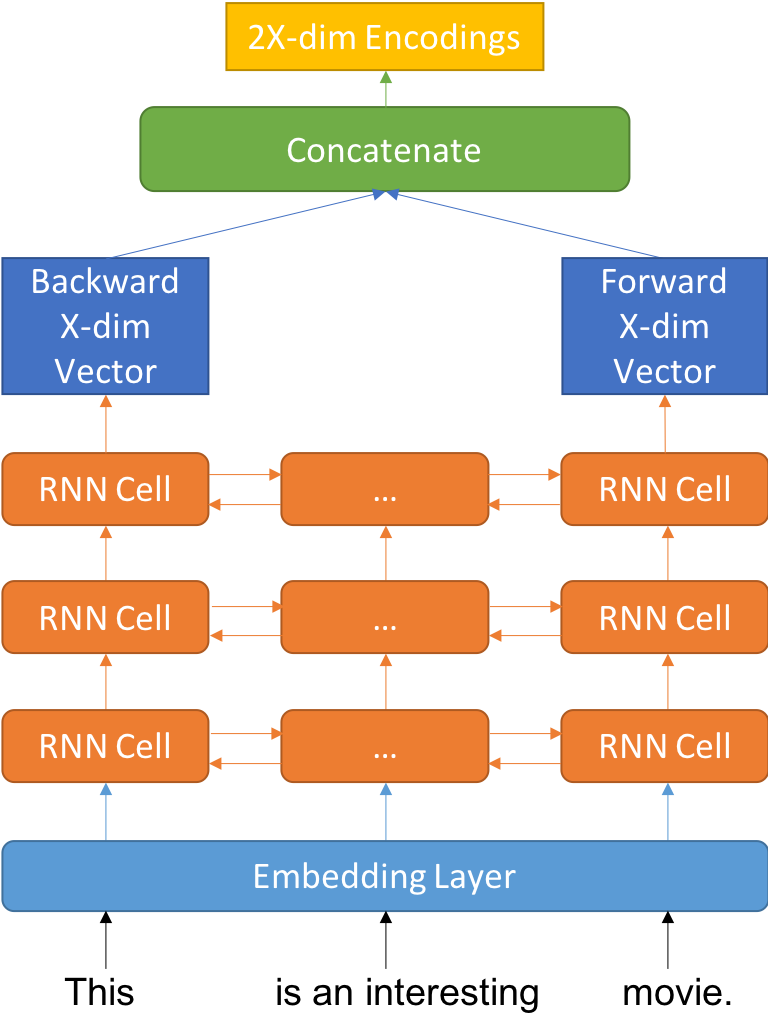
\includegraphics[width=\linewidth]{bidirect_txt_encoder.png}
  \caption{Bidirectional Encoder}
  \label{fig:bi-txt-encode}
\end{minipage}%
\hspace*{1.0in}
\begin{minipage}{0.28\textwidth}
  \centering
  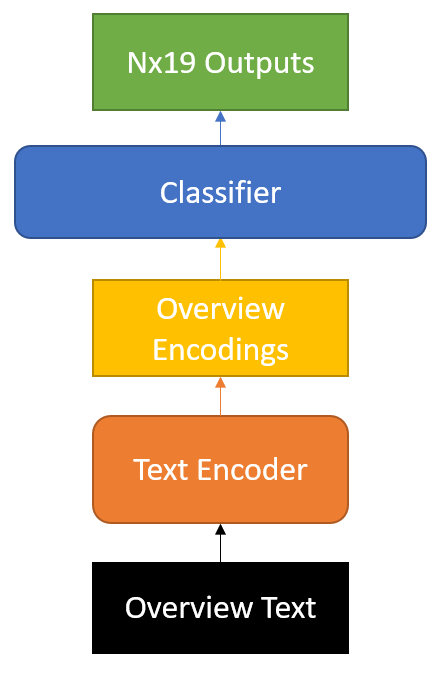
\includegraphics[width=\linewidth]{txt_network.png}
  \caption{RNN Network}
  \label{fig:text-net}
\end{minipage}%
\end{figure}

\subsection{Poster-Only CNN}

We also tried to use the posters to predict the genres. As discussed in the previous section, it is better to use transfer learning. In our project, we tried both VGG16 and ResNet-152. We first got the pre-trained weights of those two models on ImageNet and the architecture of the network is shown as the left branch of Fig.~\ref{fig:cnn}. We then threw all fully connected layers of this network (the dotted part) and used the output of the last convolution layer as poster encodings. The encoding was then fed to a similar classifier network (Fig.~\ref{fig:classifier}) like in text-only RNN. The whole architecture is shown as the right branch of Fig.~\ref{fig:cnn}

For the training, we only trained the last 2-3 convolution layers and fixed the rest of convolution layers with the ImageNet weights since we believe the network trained on ImageNet can also capture the abstract features for images in our task.

\begin{figure}[H]
\centering
\begin{minipage}{0.31\textwidth}
  \centering
  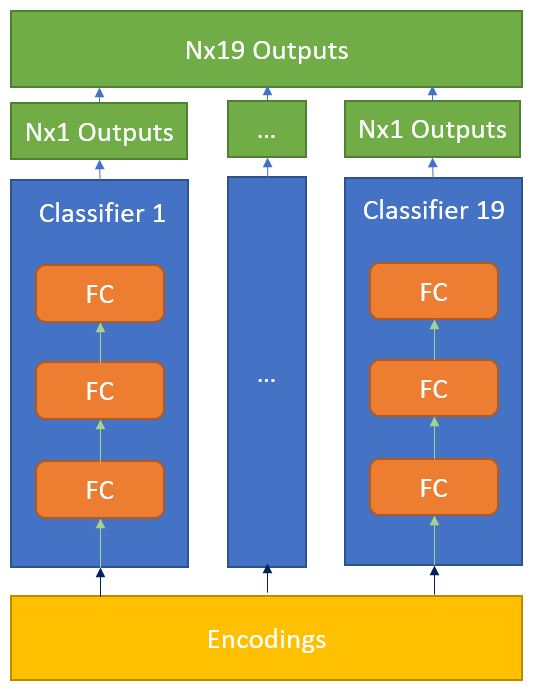
\includegraphics[width=\linewidth]{classifier.png}
  \caption{Classifier Network}
  \label{fig:classifier}
\end{minipage}%
\begin{minipage}{0.37\textwidth}
  \centering
  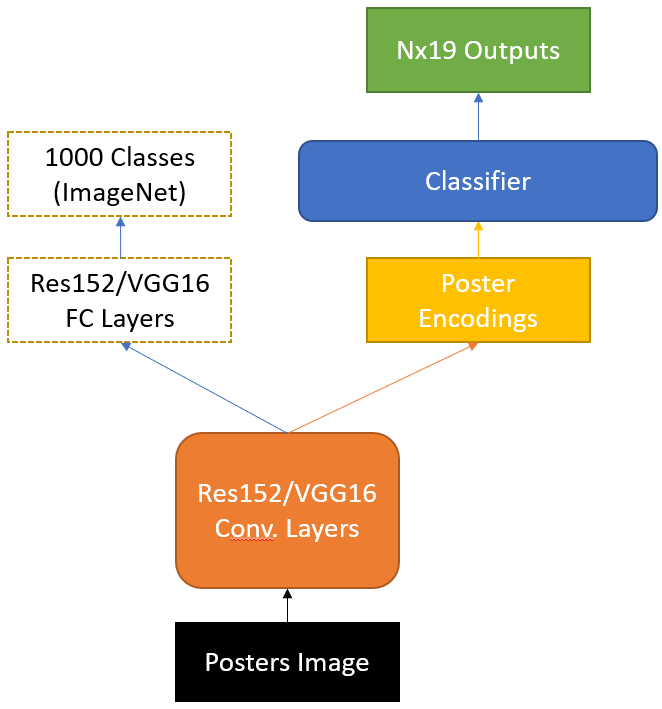
\includegraphics[width=\linewidth]{cnn.png}
  \caption{CNN Architecture}
  \label{fig:cnn}
\end{minipage}%
\begin{minipage}{0.31\textwidth}
  \centering
  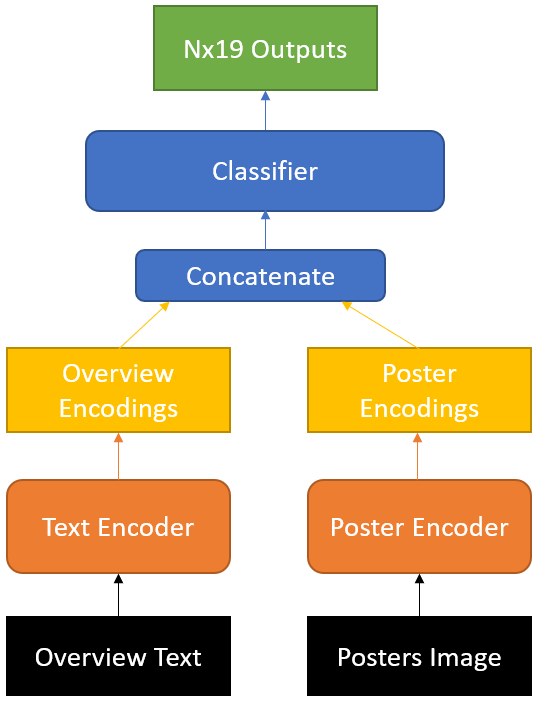
\includegraphics[width=\linewidth]{combined_net.png}
  \caption{Combined Network}
  \label{fig:combined-nn}
\end{minipage}%
\end{figure}

\subsection{RNN + CNN Combined}

We then combined the text-only RNN network with poster-only CNN network. We stacked the encodings from both networks together and then fed the encodings to 19 3-layer-fully-connected feed forward networks. The architecture is shown in Fig.~\ref{fig:combined-nn}.

Due to limitation of our GPUs, training the entire network (joint training) is very hard because it requires huge GPU RAM. Instead we {\bf fixed the encoders and only trained the classifier}.

{\bf This combined network is our final model and achives the best results in our validation and test datasets.}

\section{Project Trajectory}

According to our EDA, we found that the dataset is unbalanced in genre distribution. Therefore, we decided to use $F$-measure instead of accuracy. In addition, both texts and images seem to be useful features for classification task from EDA, so we planed to train classifiers for these individuals' features and their combined features.

For overview texts, while evaluating the conventional models, we found that different feature extraction methods affect the results, and therefore, it is natural to consider using deep neural network to learn the right representation of text data. Since text is a kind of time-series data with sequence dependencies, we applied RNNs.

For posters, we trained CNNs for the classification task. However, training good CNNs from scratch is difficult, so we used transfer learning. Our poster-only models are not as good as the text-only models and it makes sense since overview texts intuitively contain more information than posters and predicting movies' genres with only posters is very hard even for human beings.

Although poster-only models don't perform well, we believe posters contain some information that does not exist in overview texts. Therefore, we combined the poster-only network and text-only network by stacking the encodings from both networks together, and fed to another classification network. This combined model evetually achieves the best result.

\section {Results and Interpretation}

We report the results of both our baseline models (SVM and Naive Bayes) and deep learning models in the table below. Validation set (val) is used to select model and test set (test) is used to approximate our models' performance on future data.

\begin{table}[h!]
\centering
\resizebox{1.0\textwidth}{!}{%
\begin{tabular}{|c|c||c|c|c|c|} 
 \hline
 \multicolumn{2}{|c||}{Model} & $F_1$ (val) & Accuracy (val) & $F_1$ (test) & Accuracy (test) \\ [0.5ex] 
 \hline\hline
\multirow{5}{*}{\parbox{2cm}{\centering (Baseline) Conventional Models}} & SVM (bag-of-words) & 0.50 & 0.93 & 0.49 & 0.93 \\
\cline{2-6}
 & NB (bag-of-words) & 0.42 & 0.91 & 0.42 & 0.91 \\
\cline{2-6}
  & SVM (tfidf) & 0.33 & 0.93 & 0.32 & 0.93 \\
\cline{2-6}
  & NB (tfidf) & 0.14 & 0.93 & 0.14 & 0.93 \\
\cline{2-6}
  & SVM (word2vec) & 0.28 & 0.93 & 0.28 & 0.93 \\
 \hline\hline
\multirow{5}{*}{\parbox{2cm}{\centering Deep Learning Models}} & TextOnly (GRU) & 0.51 & 0.93 & 0.50 & 0.93 \\
\cline{2-6}
 &TextOnly (LSTM) & 0.53 & 0.94 & 0.51 & 0.93 \\
\cline{2-6}
 &PosterOnly (ResNet-152) & 0.45 & 0.93 & 0.43 & 0.93 \\
\cline{2-6}
 &PosterOnly (VGG16) & 0.42 & 0.92 & 0.40 & 0.92 \\
\cline{2-6}
 &\textbf{Combined (LSTM+ResNet-152)} & \textbf{0.54} & \textbf{0.95} & \textbf{0.52} & \textbf{0.94} \\
\hline
\end{tabular}}
\caption{Results on Validation Set and Test Set}
\label{table:1}
\end{table}

From Table~\ref{table:1}, we have the following observations:

1. The combined model using both plot descriptions and posters provides the best result in both validation and test set, slightly higher than RNN models with only text embedding features. {\bf All text-included deep learning models beat our baseline models (conventional models)}.

2. For the conventional machine learning models, using bag-of-words representation for text features has better predictability and it gives a result very close to our best model. The reason might be that TMDB plot discription is generally short, so simply identify certain words could be able to distinguish the genres. While using tfidf or embeddings is likely to deviate from this simple feature.  

3. Models with only poster information didn't perform well. It is very hard even for human to accurately predict simply based on posters (comparing to replying on overview texts). But combining it with text features could slightly improve our model's performance. 

\begin{figure}[H]
\centering
\begin{minipage}{0.6\textwidth}
\centering
\resizebox{1.0\textwidth}{!}{%
\begin{tabular}{|c||c|c|c|c|c|} 
 \hline
  Genre & $F_1$ & Precision &  Recall & Accuracy &     AUC \\ [0.5ex] 
 \hline\hline
Action          &  50.31\% &    61.54\% &  42.55\% &   94.73\% &  86.99\% \\
\hline
Adventure       &  36.64\% &    66.67\% &  25.26\% &   97.23\% &  87.94\% \\
\hline
Animation       &  45.61\% &    71.23\% &  33.55\% &   95.87\% &  89.01\% \\
\hline
Comedy          &  53.68\% &    61.69\% &  47.51\% &   85.73\% &  83.52\% \\
\hline
Crime           &  33.92\% &    76.32\% &  21.80\% &   96.23\% &  83.47\% \\
\hline
Documentary     &  56.14\% &    64.36\% &  49.79\% &   87.87\% &  85.37\% \\
\hline
Drama           &  60.30\% &    60.21\% &  60.40\% &   74.77\% &  79.85\% \\
\hline
\iffalse
Family          &  36.81\% &    65.22\% &  25.64\% &   96.57\% &  80.32\% \\
\hline
Fantasy         &  32.73\% &    81.82\% &  20.45\% &   97.53\% &  85.08\% \\
\hline
History         &  44.78\% &   100.00\% &  28.85\% &   98.77\% &  86.61\% \\
\hline
\fi
Horror          &  59.64\% &    80.56\% &  47.35\% &   94.77\% &  91.53\% \\
\hline
Music           &  31.65\% &    73.33\% &  20.18\% &   96.83\% &  78.04\% \\
\hline
Mystery         &  40.00\% &    95.45\% &  25.30\% &   97.90\% &  81.92\% \\
\hline
Romance         &  47.09\% &    68.99\% &  35.74\% &   93.33\% &  82.59\% \\
\hline
\iffalse
Science Fiction &  40.00\% &    83.33\% &  26.32\% &   96.50\% &  86.88\% \\
\hline
\fi
TV Movie        &  31.82\% &    70.00\% &  20.59\% &   99.00\% &  75.12\% \\
\hline
Thriller        &  46.09\% &    64.84\% &  35.76\% &   90.80\% &  86.01\% \\
\hline
\iffalse
War             &  45.45\% &   100.00\% &  29.41\% &   99.20\% &  88.00\% \\
\hline

Western         &  40.00\% &   100.00\% &  25.00\% &   99.50\% &  88.31\% \\
\hline
\fi
\end{tabular}}
\captionof{table}{Statistics for Some Genres of Combined Network (Shown in Table~\ref{table:1}) on Test Set}
\label{table:2}
\end{minipage}%
\begin{minipage}{0.39\textwidth}
  \centering
  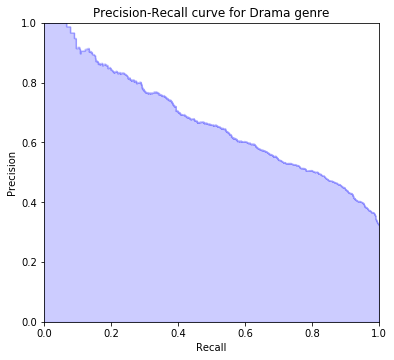
\includegraphics[width=\linewidth]{pr_drama.png}
  \caption{{\it Drama} PR curve}
  \label{fig:drama-pr}
\end{minipage}%
\end{figure}



From Table~\ref{table:2}, we have several observations:

1. All genres have reasonable $F_1$-score and AUC. Genres with larger sample sizes have better evaluation metrics (also see Fig.~\ref{fig:hist}). The classificaiton model is influenced by unbalanced data set to some degree. The discrepency between accuracy and $F_1$/AUC is a consequence of such unbalance.

2. TV Movie and Music have the worst AUC and $F_1$ score among all genres. Both of them have limited sample size and are not closely correlated with other genres. There might not be enough training data for our model to specify their unique features.

3. Human error might exist in ground truth labels since it is relatively difficult to distinguish certain correlated topics, such as horror and thriller. Therefore, considering these human error, our evaluation statistics are within reasonable range for all genres.
 
We also plot an example precision-recall (PR) curve for genre {\it Drama} as shown in Fig.~\ref{fig:drama-pr} for our combined network on test set.

\section{Conclusions}
In this project, we implemented several machine learning models to classify genres of movies using their plot descriptions and posters. We sucessfully combined these features together and made a machine learning pipeline to automatically tag the genres. The combined model with encodings from text-only RNN and poster-only CNN provided the best result among all other models. However, our best model did not outperformed the best baseline model a lot. Several proposed improvements are discussed in the next section. 

\section{Possible Future Work}
One important characteristic of our dataset is it's multi-labled. We have tried applying binary relevance method to deal with the problem (i.e. train 19 classifier each responsible for one class). However, it could be improved in several ways:
\begin{itemize}
  \item The relation among genres could be used as priors. For example, many thriller movies might also be in horror genre. Our method didn't consider such priors.
  \item For each genre, the dataset is very unbalanced. If we want to maximize $F_1$-score, we may consider using weighted loss functions or undersampling.

\end{itemize}

In addition, more combinations of hyper-parameters can be tried. We can also consider changing the training process. For example, unfix some layers of CNN or RNN during the training of the combined model. We might also consider using different embeddings (e.g. GloVe pretrained on larger dataset). In addition, We might also consider fine-tuning the embedding layer.

\input{bib.bbl}

\end{document}
